\begin{wrapfigure}{r}{0.55\textwidth}
	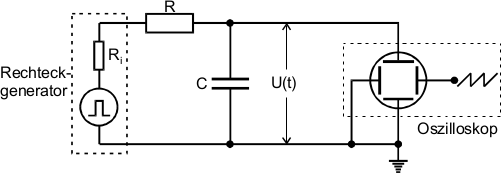
\includegraphics[width=0.5\textwidth]{Bild1.png}
	\centering
	\caption{Schaltbild zur Bestimmung der Zeitkonstanten durch Beobachten des Aufladevorgangs}
	\label{fig:Zeitkonstante}
\end{wrapfigure} \ \\
Zunächst soll die Zeitkonstante über die \textbf{Aufladekurve} des Kondensators ermittelt werden. Dazu werden mit einer Schaltung nach Abbildung \ref{fig:Zeitkonstante} die Auf- und Entladungskurven auf dem Oszilloskop visualisiert. Mit Hilfe der \textsc{Cursor}-Funktion des Oszilloskops wird dann bei einer Aufladekurve der Endwert bestimmt und für verschiedene Zeitpunkte $t_i$ der Wert $U(t_i)$ abgelesen. \\

\begin{wrapfigure}{r}{0.55\textwidth}
	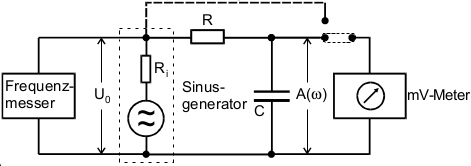
\includegraphics[width=0.5\textwidth]{Bild2.png}
	\centering
	\caption{Schaltbild zur Messung der Amplitude in Abhängigkeit zur Frequenz}
	\label{fig:Amplitude}
\end{wrapfigure} \ \\
Danach wird mit Schaltung \ref{fig:Amplitude} die \textbf{Amplitude $\bm{A}$} bestimmt. Hierfür werden am Sinus-Generator nacheinander verschiedene Frequenzen eingestellt, die einen großen Frequenzbereich überstreichen. Über die \textsc{Measure}-Funktion des Oszilloskops kann dann die jeweilige Amplitude angezeigt werden. \\

\begin{wrapfigure}{r}{0.55\textwidth}
	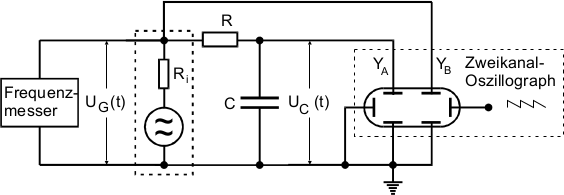
\includegraphics[width=0.5\textwidth]{Bild3.png}
	\centering
	\caption{Schaltbild zur Messung der Phasenverschiebung zwischen der Erreger- und der Kondensatorfrequenz}
	\label{fig:Phase}
\end{wrapfigure} \ \\
Die \textbf{Phasenverschiebung $\bm{\varphi}$} zwischen der Erreger- und der Kondensatorfrequenz wird mit Schaltung \ref{fig:Phase} gemessen. So können beide Spannungen am Oszilloskop angezeigt werden. Am Sinus-Generator werden dieselben Frequenzen, die zur Messung der Amplituden verwendet werden, eingestellt und mit der \textsc{Cursor}-Funktion wird direkt die Phasenverschiebung als $\Delta t$ zwischen den Nulldurchgängen gemessen. \\
\ \\
\ \\
Im letzten Versuchsteil soll die \textbf{Integratorfunktion} des RC-Kreises verifiziert werden. Dafür wird wiederum Schaltung \ref{fig:Phase} verwendet. Der Spannungsgenerator generiert eine Rechteck-, eine Sinus- und eine Dreieckspannung. Am Oszilloskop können dann die Spannung aus dem Generator und die integrierte Spannung aus dem RC-Kreis angezeigt werden.

%\begin{figure}[h!]
%	\centering
%	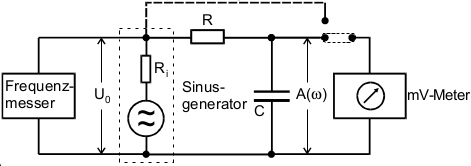
\includegraphics[width=0.6\textwidth]{Bild2.png}
%	\caption{Schaltbild zur Messung der Amplitude in Abhängigkeit zur Frequenz}
%	\label{fig:Amplitude}
%\end{figure} \\
%\begin{figure}[h!]
%	\centering
%	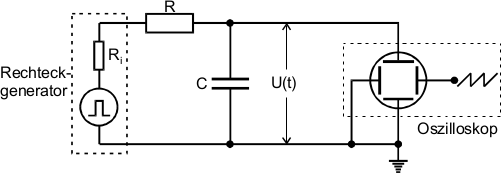
\includegraphics[width=0.6\textwidth]{Bild1.png}
%	\caption{Schaltbild zur Bestimmung der Zeitkonstanten durch Beobachten des Aufladevorgangs}
%	\label{fig:Zeitkonstante}
%\end{figure} \\
%\begin{figure}[h!]
%	\centering
%	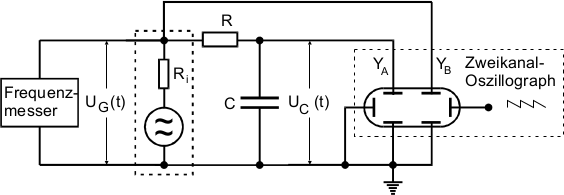
\includegraphics[width=0.6\textwidth]{Bild3.png}
%	\caption{Schaltbild zur Messung der Phasenverschiebung zwischen der Erreger- und der Kondensatorfrequenz}
%	\label{fig:Phase}
%\end{figure}